\documentclass[12pt]{article}
\usepackage[english]{babel}
\usepackage[utf8x]{inputenc}
\usepackage{amsmath}
\usepackage{graphicx}
\usepackage[colorinlistoftodos]{todonotes}

\begin{document}

\begin{titlepage}

\newcommand{\HRule}{\rule{\linewidth}{0.5mm}} % Defines a new command for the horizontal lines, change thickness here

\center % Center everything on the page
 
% Heading
\textsc{\LARGE Seneca College}\\[1.5cm]
\textsc{\Large School of Information and Communications Technology}\\[0.5cm]
\textsc{\large PC Hardware I}\\[0.5cm]

% Title
\HRule \\[0.4cm]
{ \huge \bfseries Project Proposal}\\[0.4cm] % Title of your document
\HRule \\[1.5cm]
 
% Author
\begin{minipage}{0.4\textwidth}
\begin{flushleft} \large
\emph{Author:}\\
Jiuxiang (Leon) \textsc{Lin}
Nischay \textsc{LASTNAME}
Mackenzie \textsc{Hodd}
\end{flushleft}
\end{minipage}
~
\begin{minipage}{0.4\textwidth}
\begin{flushright} \large
\end{flushright}
\end{minipage}\\[2cm]

{\large \today}\\[2cm]


\includegraphics{logo.png}\\[1cm]

\vfill

\end{titlepage}


% Begin body of article
\begin{abstract}
Proposal for the HWD101 Group Project.	
\end{abstract}

\section{Group Members}

\begin{tabular}{| c | c | c | c |}
\hline
\textbf{Name} & \textbf{Student Number} & \textbf{Email} & \textbf{Responsibility} \\\hline
Jiuxiang Lin & 124462185 & jlin164@myseneca.ca & Tech \\\hline
Nischay & 123456789 & nischay@myseneca.ca & Presenter \\\hline
\end{tabular}

\section{Introduction}

As we move into the new era of technology, the demand of security, accessibility and convenience is getting higher and higher. Enterprise class solutions are very capable with outstanding quality. However, as an ordinary Internet user, it is very had for an individual to afford the enterprise grade services.

\vfill

\section{Topology Design}

\subsection{Option 1}

The raspberry pi will have the following roles on the network:

\begin{enumerate}
\item OpenConnect Server
\item Pi-Hole
\item FreeRADIUS
\end{enumerate}

\begin{center}
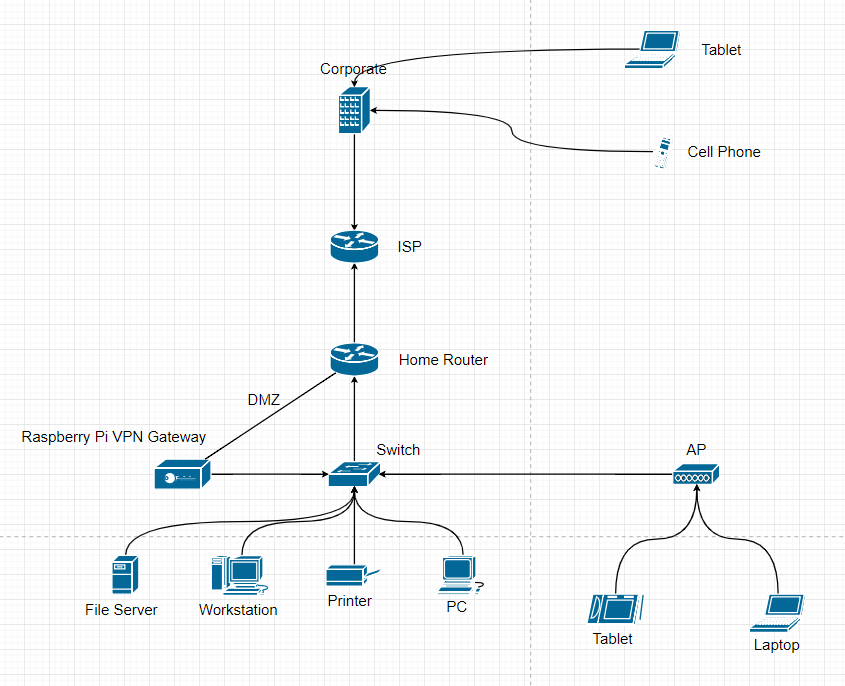
\includegraphics[scale=0.6]{topology.png}\\[1cm]
\end{center}

\subsection{Option 2}

The raspberry pi will have the following roles on the network:

\begin{enumerate}
\item OpenConnect Server
\item Pi-Hole
\item FreeRADIUS
\item Router
\item DHCP Server
\end{enumerate}

\section{Materials Needed}

The follow is a list of all the components and devices that are expected to be used in this project. Some of these devices are enterprise level devices. They are used not because this project require excessive computing power nor throughput. They are used since Jiuxiang Lin is already in possession of these devices.

\begin{enumerate}
\item Raspberry pi
\item Cisco C819G (Router)
\item Cisco WS-C3750 (Swich)
\item Laptop / Smart phone (as terminal devices)
\item Ethernet cables
\item Other minor accessories
\end{enumerate}

\end{document}